
%% CLASS MANUAL FOUND at http://blog.poormansmath.net/latex-class-for-lecture-notes/ %%
%% CLASS AUTHOR Stefano Maggiolo %%
\documentclass[english,course]{Notes}

\title{MATHEMATICS 1S}
\subject{Mathematics}
\author{Joao Almeida-Domingues}
\email{2334590D@student.gla.ac.uk}
\speaker{Dr. Andrew Wilson}
\date{07}{01}{2019}
\dateend{24}{05}{2019}
\place{University of Glasgow}

 %%%%% GENERAL MATHEMATICAL NOTATION SHORTCUTS %%%%%
 
\newcommand{\n}{\mathbb{N}}
\newcommand{\z}{\mathbb{Z}}
\newcommand{\q}{\mathbb{Q}}
\newcommand{\cx}{\mathbb{C}}
\newcommand{\real}{\mathbb{R}}
\newcommand{\field}{\mathbb{F}}
\newcommand{\ita}[1]{\textit{#1}}
\newcommand{\oneton}{\{1,2,3,...,n\}}
\newcommand\ef{\ita{f} }
\newcommand\inv[1]{#1^{-1}}
\newcommand\setb[1]{\{#1\}}
\newcommand\en{\ita{n }}

%\renewcommand\qedsymbol{QED} %to use QED instead of square


%%%%%%%%%%%%%%%%PACKAGES%%%%%%%%%%%%%%%%%%%%%%%%%%%%%
\usepackage{lipsum}  
\usepackage{amsmath,amsthm,amssymb,graphicx,mathtools,tikz,pgfplots,minibox} %maths
\pgfplotsset{compat=1.16}
\usepackage{hyperref,framed,color,fancybox} %layout
% framed :  \begin{shaded,frame,snugshade or leftbar} \definecolor{shadecolor}{rgb}{XYZ} to change color
%fancybox: \shadowbox,ovalbox or doublebox
%%%%%%%%%%%%%%%%%%%%%%%%%%%

%%%CLASS SHORTCUTS%%%%
%\lecture{day}{month}{year} for margin note 
%\begin{theorem} sdfsdf\end{theorem}
%\begin{proposition} dfsdfs\end{proposition}
%\begin{lemma} dsfsd \end{lemma} %lem
%\begin{corollary} f ffew \end{corollary}
%\begin{definition} fwewef w \end{definition} %defn
%\begin{example} feww e\end{example} %ex
%\begin{exercise} wefwe \end{exercise}
%\begin{remark} wef we \end{remark} %rem
%\begin{fact} wefe \end{fact}
%\begin{problem} wef ew \end{problem}
%\begin{conjecture} ewfew \end{conjecture}
%\begin{claim} few w \end{claim}
%\begin{notation} fewf \end{notation} %nota

\begin{document}
\newpage

\section{Vectors}

\subsection{Generalities}

\lecture{07}{01}{2019}

\defn{A scalar}{is a one-component quantity that is invariant under rotations of the coordinate system, which describes the magnitude of something}

\defn{A vector}{ is a two-component quantity, with magnitude (a positive real number) and direction}

\rem{If a vector has both a magnitude and direction of $0$, then that vector is  the zero vector. The zero vector can be thought as having no direction, or all directions}

\defn{Equality:}{ Two vectors are equal if they have the same magnitude and the same direction\label{def:eq}}

\rem{Every vector is unique}

\proofs{ Let $\vc{u}, \vc{v}$ be two vectors with magnitude $\lambda$ and the same direction. Hence by \ref{eq} , $\vc{u} = \vc{v}$}


\nota{ Generally, in printed text $\overrightarrow{v} \text{ or } \ \vc{v}$. Handwritten \underline{$v$}. Magnitude $\vc{|v|}$}

\defn{Unit vector}{is a vector of magnitude 1. There is exactly one for any given direction}
\nota{Generally, for a given vector $\vc{v} \ , \ \hat{\vc{v}}$}

\prop{Parallelogram }{$\overrightarrow{AB} = \overrightarrow{DC}$\ , i.e Traversing left-up is the same as up-right}
\proofs{It follows from the fact that the opposite sides of a parallelogram are parallel and of equal length. Hence they are equal, by \ref{eq}}

\prop{Negative vectors }{$\overrightarrow{AB} = u \iff \overrightarrow{BA} = -u$}
\proofs{It follows from the fact that they have the same magnitude but opposite directions}

\prop{Zero vector }{$\overrightarrow{AA} = 0$}
\proofs{For any point $A, |AA| = 0$ and so $\overrightarrow{AA} = 0$}

\subsection{Addition and Scalar Multiplication}

\defn{Addition}{Let $\vc{u} = \overrightarrow{PQ} \ , \ \vc{v} = \overrightarrow{QR}. \vc{u} + \vc{v} = \overrightarrow{PR}$. \ita{nose-to-tail}}

\rem{As per usual subtraction is simply, $\vc{u} + (-\vc{v})$}

\defn{Scalar Multiplication}{For a vector $\vc{u}$, and a scalar $\lambda$. $\lambda\vc{u}$ scales the vector's magnitude  by $\lambda$, and if $\lambda<0$ inverts its direction}

\lecture{8}{01}{2019}
\subsubsection{Properties of Addition and Multiplication}
\prop{Commutative }{$\vc{u} + \vc{v} = \vc{v} + \vc{u}$}
\proofs{
\begin{align*}
	 \vc{u} + \vc{v} & = [u_1, u_2 , \dots , u_n] + [v_1 , v_2 , \dots , u_n] \\
	 & = [u_1 + v_1 , u_2 + v_2 , \dots , u_n + v_n] \text{  \ita{vector addition}} \\
	 & = [v_1 + u_1, v_2 + u_2 , \dots , v_n + u_n] \text{  \ita{commutative adition of real numbers}} \\
	 & = [v_1 , v_2 , \dots , v_n] + [u_1, u_2 , \dots , u_n] \\
	 & = \vc{v} + \vc{u}
\end{align*}
}


\prop{Associative }{$(\vc{u} + \vc{v}) + \vc{w} = \vc{u} + (\vc{v} + \vc{w})$}
\proofs{
\begin{align*}
	(\vc{u} + \vc{v}) + \vc{w} & = ([u_1, u_2 , \dots , u_n] + [v_1 , v_2 , \dots , v_n]) + [w_1 , w_2 , \dots , w_n] \\
	 & = [u_1 + v_1 , u_2 + v_2 , \dots , u_n + v_n]  + [w_1 , w_2 , \dots , w_n]   \mathbf(1.10) \\
	 & = [(u_1 + v_1) + w_1, (u_2 + v_2) + w_2, \dots , (u_n + v_n) + w_n] \text{  \ita{commutative property of scalars}} \\
	 & = [u_1 + (v_1 + w_1), u_2 + ( v_2 + w_2), \dots , u_n + (v_n + w_n)] \text{  \ita{associative addition of real numbers}} \\
	 & = [u_1 , u_2 , \dots , u_n] + [v_1 + w_1 , v_2 + w_2 , \dots , v_n + w_n]  \\
	 & = \vc{u} + \vc{v} + \vc{w}
\end{align*}
}

\prop{Distributive }{$\lambda(\vc{u} + \vc{v}) = \lambda\vc{u} +\lambda\vc{v}$}
\proofs{
\begin{align*}
	\lambda(\vc{u} + \vc{v}) & = \lambda([u_1 + v_1 , u_2 + v_2 , \dots , u_n + v_n]   \text{  \ita{vector addition}} \\ 
	& = [\lambda(u_1 + v_1) , \lambda(u_2 + v_2) , \dots , \lambda(u_n + v_n)] \text{  \ita{scalar multiplication} }\\
	& = [\lambda u_1 + \lambda v_1 , \lambda u_2 + \lambda v_2 , \dots , \lambda u_n + \lambda v_n] \text{  \ita{distributive for real numbers}} \\
	& = \lambda\vc{u} + \lambda\vc{v}
\end{align*}
}

\newpage
\proofs{ \ita{2 , by a diagram} \\

Let $\vc{u} , \vc{v}$ be two non-zero vectors, and A, B, C be 3 distinct points. Then:

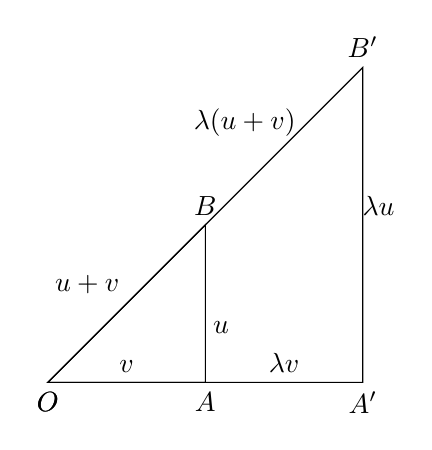
\begin{tikzpicture}
\centering
\draw (0,0) node[anchor=north]{$O$}
  -- (2,0) node[anchor=north]{$A$}
  -- (2,2) node[anchor=south]{$B$}
    -- cycle;
    \draw
  -- (0.5,1) node[anchor=south]{$\vc{u} + \vc{v}$}
  -- (2.2,0.5) node[anchor=south]{$\vc{u}$}
  -- (1,0) node[anchor=south]{$\vc{v}$};


\draw (0,0) node[anchor=north]{$O$}
  -- (4,0) node[anchor=north]{$A'$}
  -- (4,4) node[anchor=south]{$B'$}
  -- cycle;
  \draw
    -- (2.5,3) node[anchor=south]{$\lambda(\vc{u} + \vc{v})$}
  -- (4.2,2) node[anchor=south]{$\lambda\vc{u}$}
  -- (3,0) node[anchor=south]{$\lambda\vc{v}$};
  \end{tikzpicture}

Let the "prime" triangle represent a $\lambda$ fold enlargement of the original triangle representing the original vectors and their addition. Hence we have that,

\begin{align*}
OB' = \lambda(\vc{u} + \vc{v}) & = OA' + A'B' \\
& = \lambda\vc{v} + \lambda\vc{u}
\end{align*}
}







\subsection{Parallel and Position vectors}

\defn{Parallel:}{ Let $\vc{u} \ , \ \vc{v}$ be two non-zero vectors. Then, 
$\vc{v}$ is parallel to $\vc{u}$ \ita{iff} $\vc{v} = \lambda\vc{u}$ (i.e. if they share the same or opposite directions) and $\hat{\vc{u}} = \frac{1}{|\vc{u}|}\vc{u}$}

\rem{The non-zero vector is parallel to all vectors}

\proofs{ The first part of the definition is self-evident as any scalar multiple of a vector will only alter its magnitude and/or reverse its direction. For the second part, we have that:

$$ \bigg|\frac{1}{|\vc{u}|}\vc{u}\bigg| = \frac{1}{|\vc{u}|}|\vc{u}| = 1 $$

Hence, we've shown that $\frac{1}{|\vc{u}|}|\vc{u}|$ is a unit vector of $\vc{u}$, which means that it only varies in magnitude, and is therefore parallel.
}

\defn{Position:}{Let $O$ denote the origin, the vector from $O$ to any point $P$ ($\overrightarrow{OP}$) is called the position vector. For any points  $A \text{ and } B , \overrightarrow{ AB } = \vc{b} -  \vc{a}$}

\nota{ $\vc{r}_p$}

\proofs{ \\

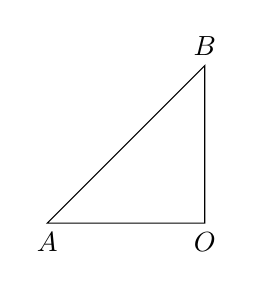
\begin{tikzpicture}
\centering
\draw (0,0) node[anchor=north]{$A$}
  -- (2,0) node[anchor=north]{$O$}
  -- (2,2) node[anchor=south]{$B$}
  -- cycle;
\end{tikzpicture} 
\ \ \ \ \ \  $
\begin{aligned} \overrightarrow{ A B } & = \overrightarrow { A O } + \overrightarrow { O B } \\ & = ( - \mathbf { a } ) + \mathbf { b } \\ & = \mathbf { b } - \mathbf { a } \end{aligned}$
}
\subsection{Collinearity and the section formula}

\defn{Collinear}{points, lie on a straight line}

\rem{One can test wether points are collinear by finding if their directed line segments, i.e. the vector formed starting at a point and ending at the other, are parallel.}

\ex{ Let $\overrightarrow{AB} = \vc{u} , \overrightarrow{BC} = 2\vc{u} , \overrightarrow{AC} = \vc{u} + \vc{2u} = \vc{3u}$. Hence they are all parallel to $\vc{u}$, it follows then that they are collinear.}

\rem{ $$ AB : BC = \beta : \alpha \implies \alpha \overrightarrow{AB} = \overrightarrow{BC} $$ 

Setting $\lambda = \frac{\beta}{\alpha}$,

$$ \overrightarrow{AB} = \lambda\overrightarrow{BC} \ \ \ AB : BC = \lambda : 1 $$

Since $A , B \text{ and } C$ are collinear, we can deduce the distance between the points using their ratio \Big($\lambda = \tfrac{|AB|}{|BC|}$\Big). Furthermore, for $\lambda > 0 $ we have that the vectors have the same direction,  hence $B$ lies between $A$ and $C$. Note however that this is not true for $\lambda < 0$ \\} 


\begin{tikzpicture}
\draw (0,0) node[anchor=north]{$A$}
  -- (2,0) node[anchor=north]{$B$}
  node[pos=0.5]{$>$}
  -- (5,0) node[anchor=north]{$C$}
    node[pos=0.5]{$>$}
  	(6,0) node[anchor=north]{$A$}
  -- (8,0) node[anchor=north]{$C$}
  node[pos=0.5]{$>$}
  node[pos=1.5]{$<$}
  -- (10,0) node[anchor=north]{$B$};
   
\end{tikzpicture} 

*******CLARIFY POST LECTURE********




\prop{Section Formula \label{secForm}}{ Let $A, B \text{ and } P$ be collinear points, s.t:

$$ AP : PB = m : n $$

Then, $P$ has position vector $$ \vc{p} = \frac{m\vc{b} + n\vc{a}}{m + n} $$

\begin{tikzpicture}
\draw (2,0) -- (10,0)
(4,0) node[anchor=north]{$A$}
(5,0) node[anchor=south]{$m$}
(7,0) node[anchor=north]{$P$}
(8,0) node[anchor=south]{$n$}
(9,0) node[anchor=north]{$B$};

\end{tikzpicture}
 }

\proofs{ 
\begin{align*}
n\overrightarrow{AP} &= m \overrightarrow{PB} \\
n(\vc{p} - \vc{a}) &= m(\vc{b} -\vc{p}) \\
(m+n)\vc{p} &= m\vc{b} + n\vc{a} \\
\vc{p} &= \frac{m\vc{b} + n\vc{a}}{m + n}
\end{align*}}

\begin{corollary}{The midpoint of $AB$ has position vector $\tfrac{1}{2}(\vc{a} + \vc{b})$ \marginpar{special case of \ref{secForm}, where $m = n = 1$}}\end{corollary}

\newpage
\section{Logical Matters \& Proof}

\defn{Direct Proof}{It consists of an argument that starts from the hypothesis and by a sequence of logical steps ends at the conclusion}

\rem{A common misconception is starting from the conclusion and finding something "true", by using both sides of the equation simultaneously}

\ex{Prove that the product of two odd integers is also odd}

\proofs{ Let $a, b$ be arbitrary odd integers. Then a $ a = 2k + 1$ and $b = 2l + 1$, for some $k, l \in \z$. Hence, \\

\begin{align*}
	ab &= (2k + 1)(2l + 1) \\
	&= 4kl + 2k + 2l + 1 \\
	&= 2(2kl + k + l) + 1
\end{align*}

Therefore, since $2kl + k + l \in \z$, $ab$ is odd.}


\end{document}